\chapter{Despliegue por defecto.}

El despliegue de ATLAS en Docker es muy sencillo y está bien documentado en el  \href{https://github.com/OHDSI/Broadsea}{repositorio de github} de Broadsea. De hecho, la propia organización considera Broadsea la manera más sencilla de instalar (y actualizar) Docker. Igualmente, en este manual detallaremos nuevamente los pasos para la configuración y despliegue de la herramienta.

\section{Requisitos para el despliegue}

\begin{enumerate}
    \item Descargar e instalar Docker. Lo más sencillo es seguir las instrucciones de la \href{https://docs.docker.com/engine/install/}{página web oficial} para la descarga y seguir la configuración por defecto para la instalación.
    
    \item Descargar e instalar Git. Lo más sencillo es seguir las instrucciones de la \href{https://git-scm.com/downloads}{página web oficial} para la descarga y seguir la configuración por defecto para la instalación.
\end{enumerate}

\section{Deployment}
\begin{enumerate}
    \item El primer paso para desplegar ATLAS es clonar localmente el repositorio de GitHub de Broadsea. Una forma rápida de hacerlo es, desde la terminal, introducir la siguiente línea.

\begin{lstlisting}[language=sh]
        git clone https://github.com/OHDSI/Broadsea.git
\end{lstlisting}

    \item El segundo paso, es desplegar el contenedor docker. Para ello, desde la terminal, nos situamos en la carpeta donde se ha copiado el repositorio de github de Broadsea. Podemos utilizar el comando cd con la ruta al repositorio local.

\begin{lstlisting}[language=sh]
        cd ruta\del\repositorio\Broadsea\local
\end{lstlisting}

    Una vez nos encontramos en la carpeta raíz del repositorio, ejecutamos el siguiente comando, que instalará el contenedor docker en nuestro ordenador.

\begin{lstlisting}[language=sh]
    docker compose pull && docker-compose --profile default up -d
\end{lstlisting}

\end{enumerate}

%---------------------------------------------------------------
\section{Comprobación de despliegue correcto} 

Podemos comprobar que se ha instalado correctamente el contenedor de Broadsea en nuestro ordenador de distintas formas, así como comprobar su correcto despliegue y ejecución e instalación de parámetros de configuración. En esta sección vamos a abordar todos estos puntos.

\begin{enumerate} 

    \item La forma más sencilla de interactuar con el contenedor de Broadsea es a través de Docker Desktop. Ejecutando dicho programa, en la sección \textit{"containers"} se muestran todos los contenedores que están corriendo en el equipo. En este caso, debe aparecer un multi-contenedor llamado "broadsea" que contenga seis contenedores, tal y como se muestra en la Figura \ref{fig:dockerDesktop}.
    
    Mediante el panel de control de Docker se puede iniciar, pausar o detener cada contenedor (o todos a la vez) fácilmente y en cualquier momento. Por esto se dice que Broadsea es \textit{a-la-carte}.
    
\begin{figure}[H]
    \centering
    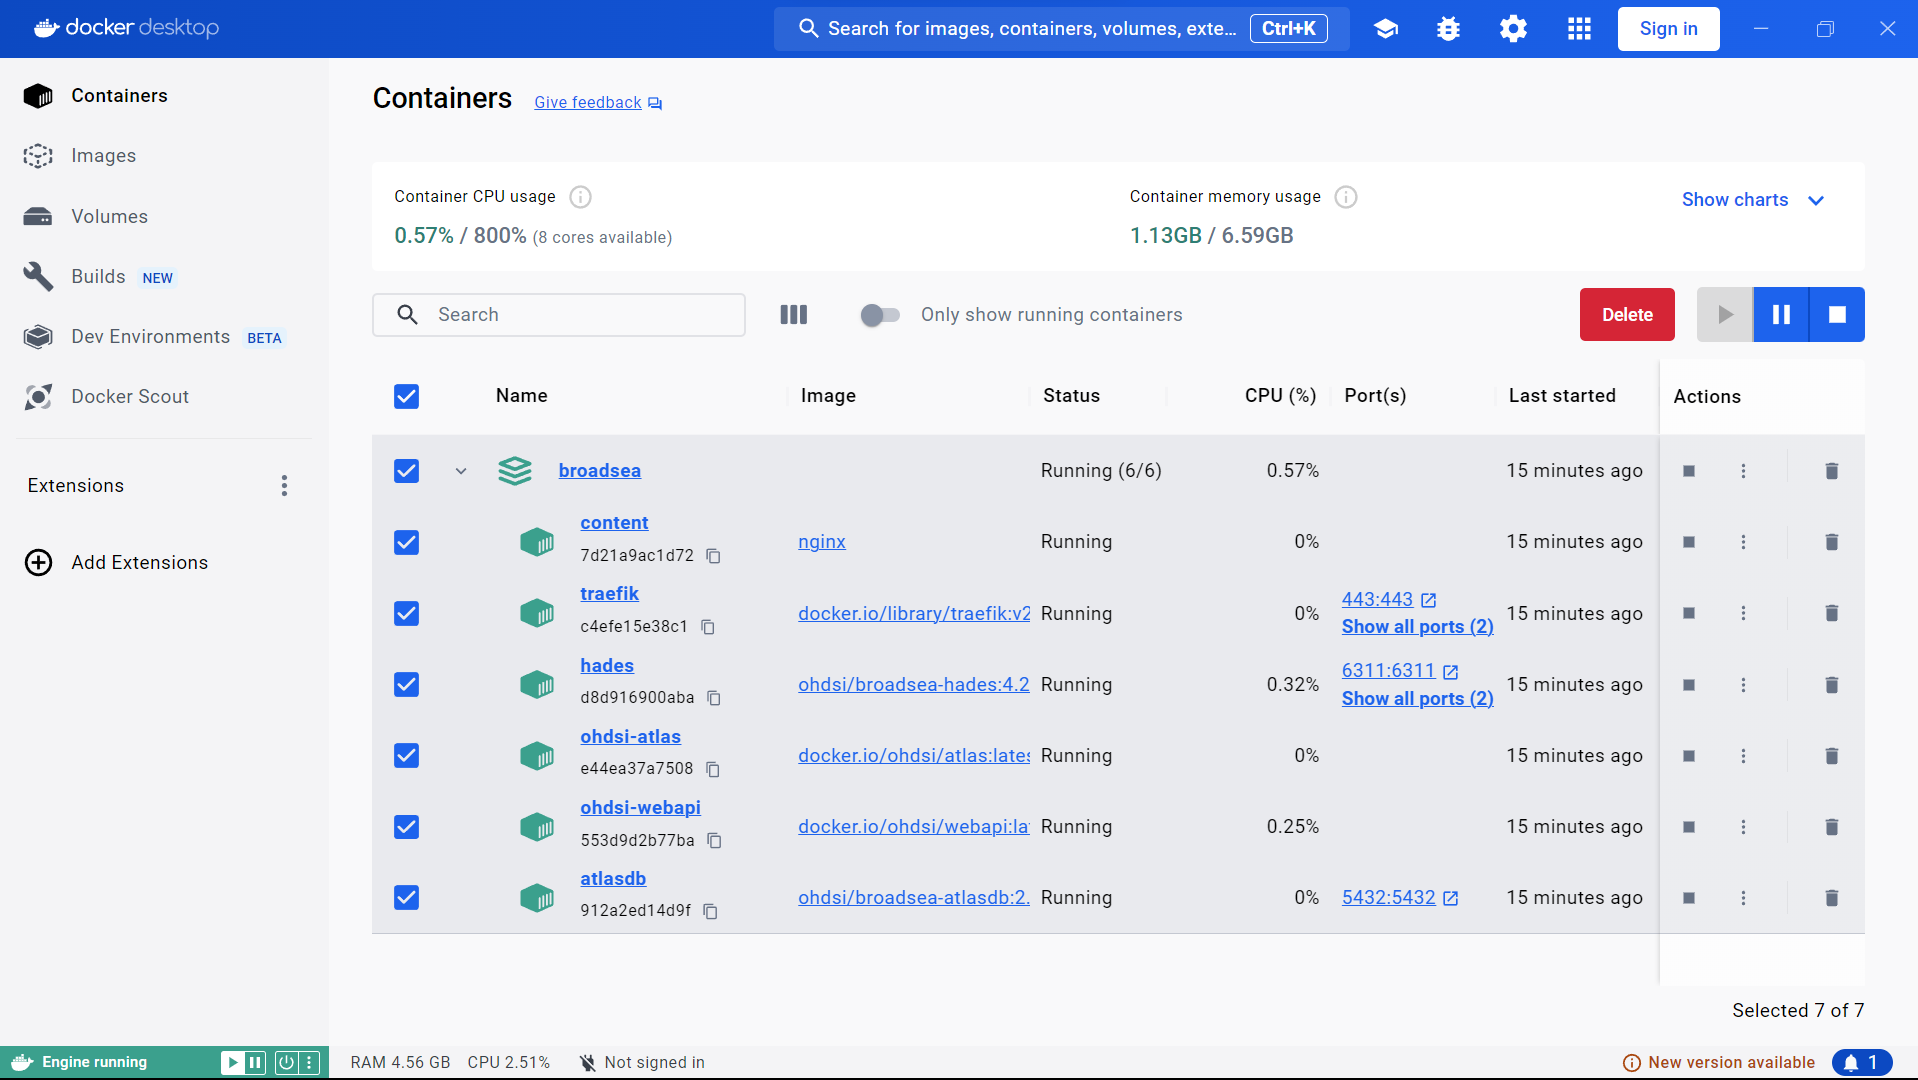
\includegraphics[width=0.90\textwidth]{figures/dockerDesktop.png}
    \caption{Captura de pantalla del contenedor Broadsea en Docker Desktop}
    \label{fig:dockerDesktop}
\end{figure}

    \item Otra forma de comprobar que Docker está ejecutando el contenedor correctamente en nuestro dispositivo es mediante la terminal, a través del comando ''docker ps'', que muestra un listado de todos los contenedores que se están ejecutando. De esta forma deberían mostrarse los seis contenedores pertenecientes a broadsea, tal y como se muestra en la Figura \ref{fig:dockerCMD}

\begin{figure}[H]
    \centering
    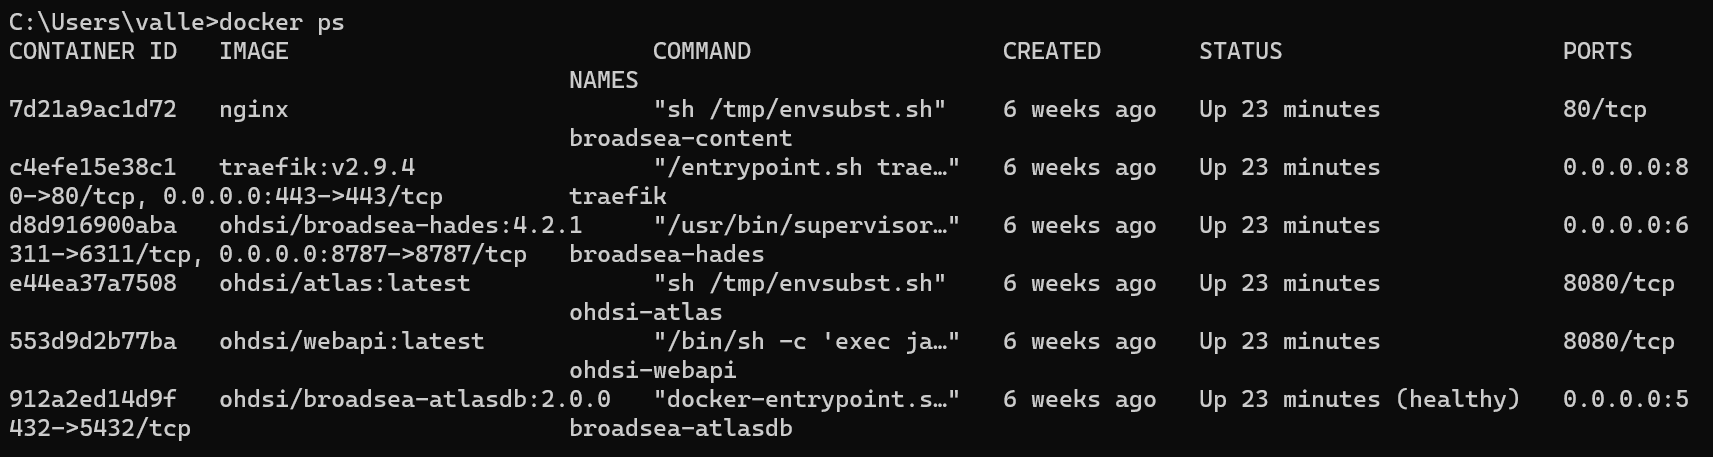
\includegraphics[width=0.90\textwidth]{figures/dockerCMD.png}
    \caption{Captura de pantalla del comando ''docker ps'' en la terminal.}
    \label{fig:dockerCMD}
\end{figure}
    
    \item Por otro lado, podemos comprobar los parámetros y configuraciones relevantes de los contenedores instalados en los archivos "docker-compose" y ".env" que se encuentran en la carpeta local del repositorio clonado de github de Broadsea, como se muestra en la Figura \ref{fig:envFile}

    \begin{figure}[H]
    \centering
    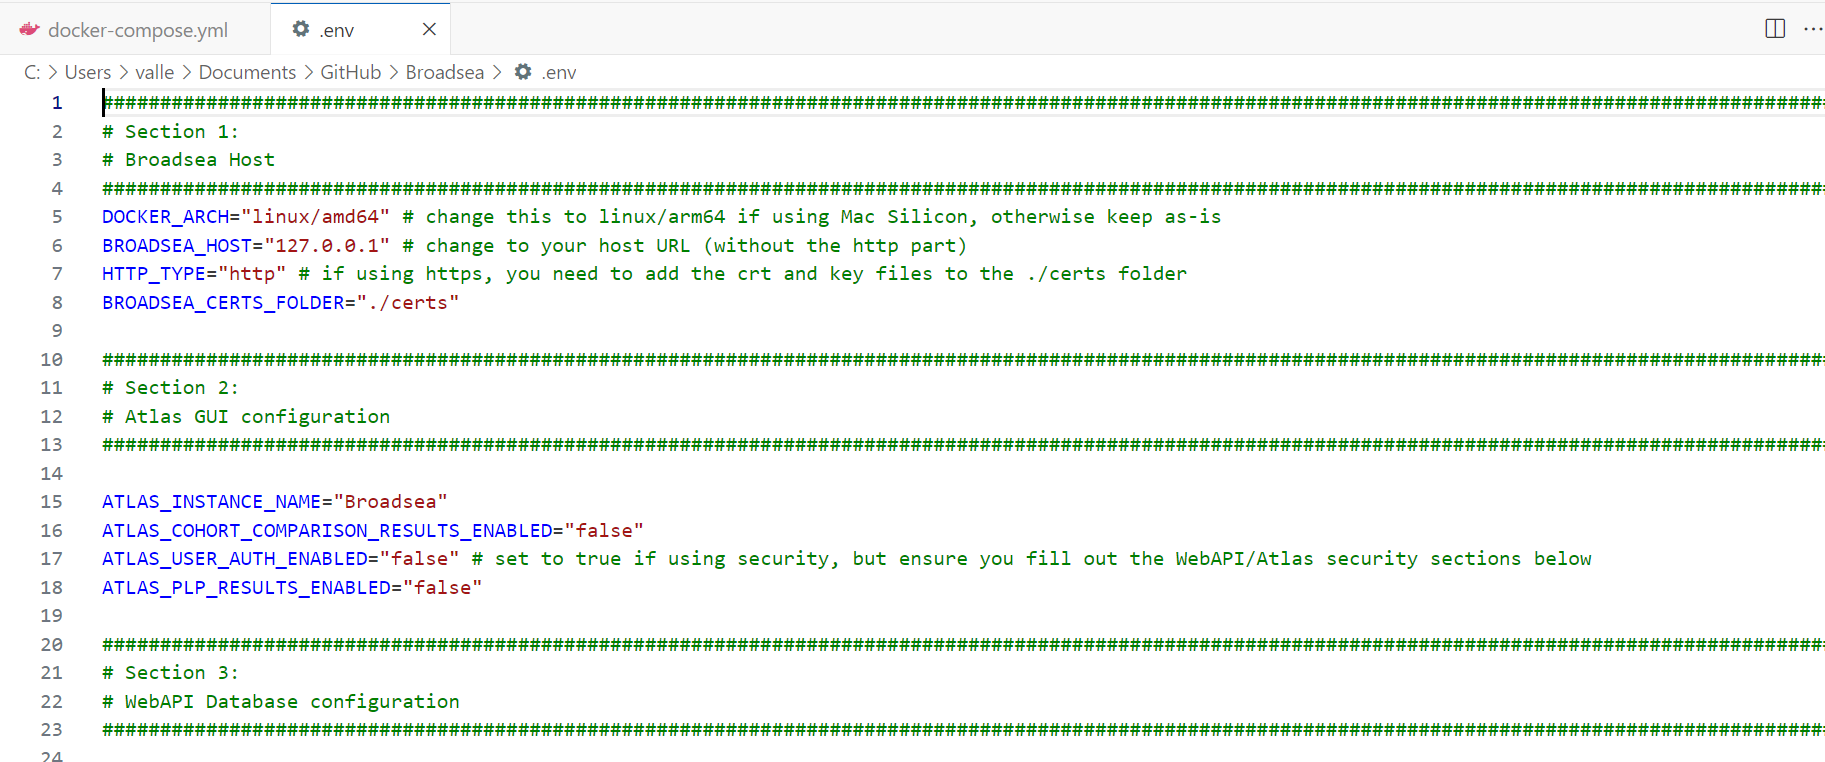
\includegraphics[width=0.90\textwidth]{figures/envFile.png}
    \caption{Captura de pantalla del archivo .env del repositorio Broadsea.}
    \label{fig:envFile}
\end{figure}

    \item Por último, para acceder a los servicios de Broadsea hay que abrir en nuestro navegador web (Chrome recomendado) el servidor en el que se alojan los servicios. Por defecto, Broadsea viene configurado para alojarse en el localhost (ya sea en el puerto 0.0.0.0 o 127.0.0.1). Podemos comprobar el puerto exacto revisando la configuración según las intrucciones del punto anterior.

    En este caso, el servidor de Broadsea se aloja en la dirección 127.0.0.1, tal y como se muestra en la Figura \ref{fig:broadseaCap}. Es interesante notar que Broadsea permite el acceso interactivo a la herramienta Atlas, que es la que nos interesa en este caso, pero también a Ares y a Hades, otras dos herramientas muy relacionadas.

\begin{figure}[H]
    \centering
    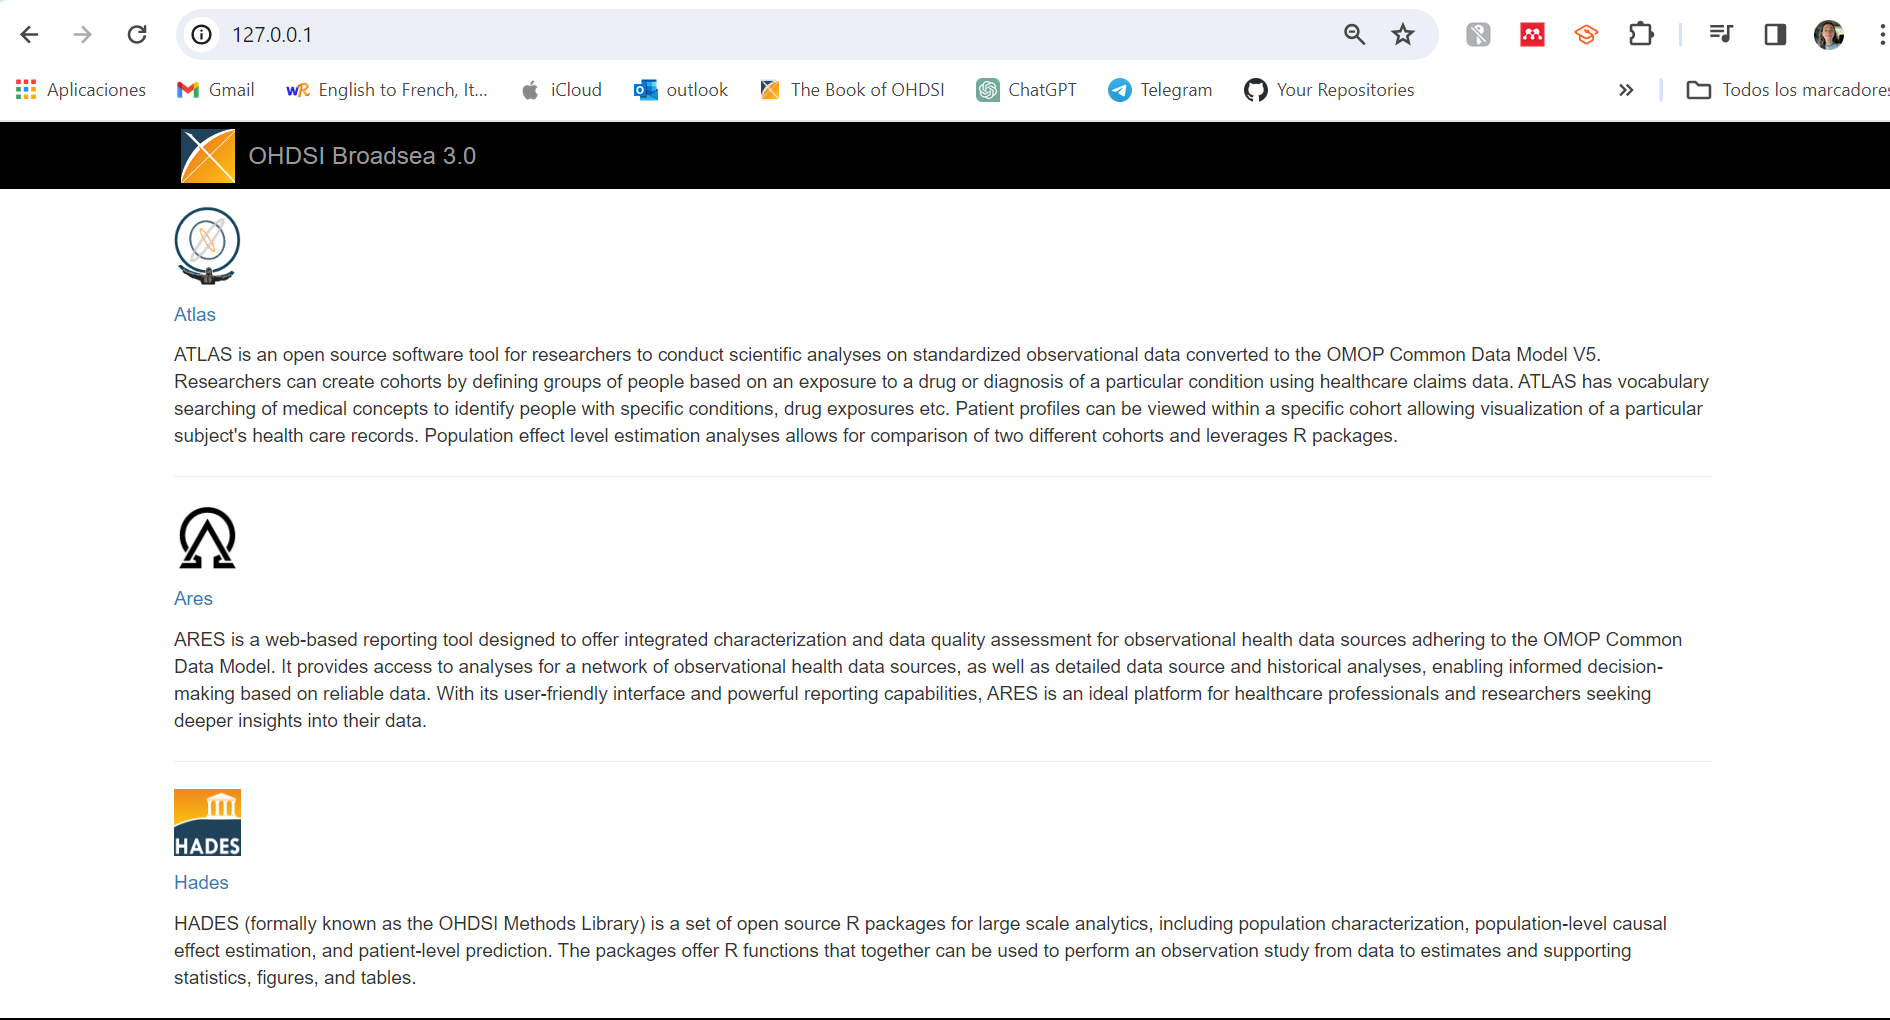
\includegraphics[width=0.90\textwidth]{figures/broadseaCap.png}
     \caption{Captura de pantalla del servidor Broadsea ejecutado en Chrome}
    \label{fig:broadseaCap}
\end{figure}

    La ejecución de ATLAS en Broadsea es similar a ATLAS demo, aunque con algunas diferencias. En primer lugar, Broadsea solo ejecuta, por defecto, una base de datos, que es la base de datos de Eunomia.

\begin{figure}[H]
    \centering
    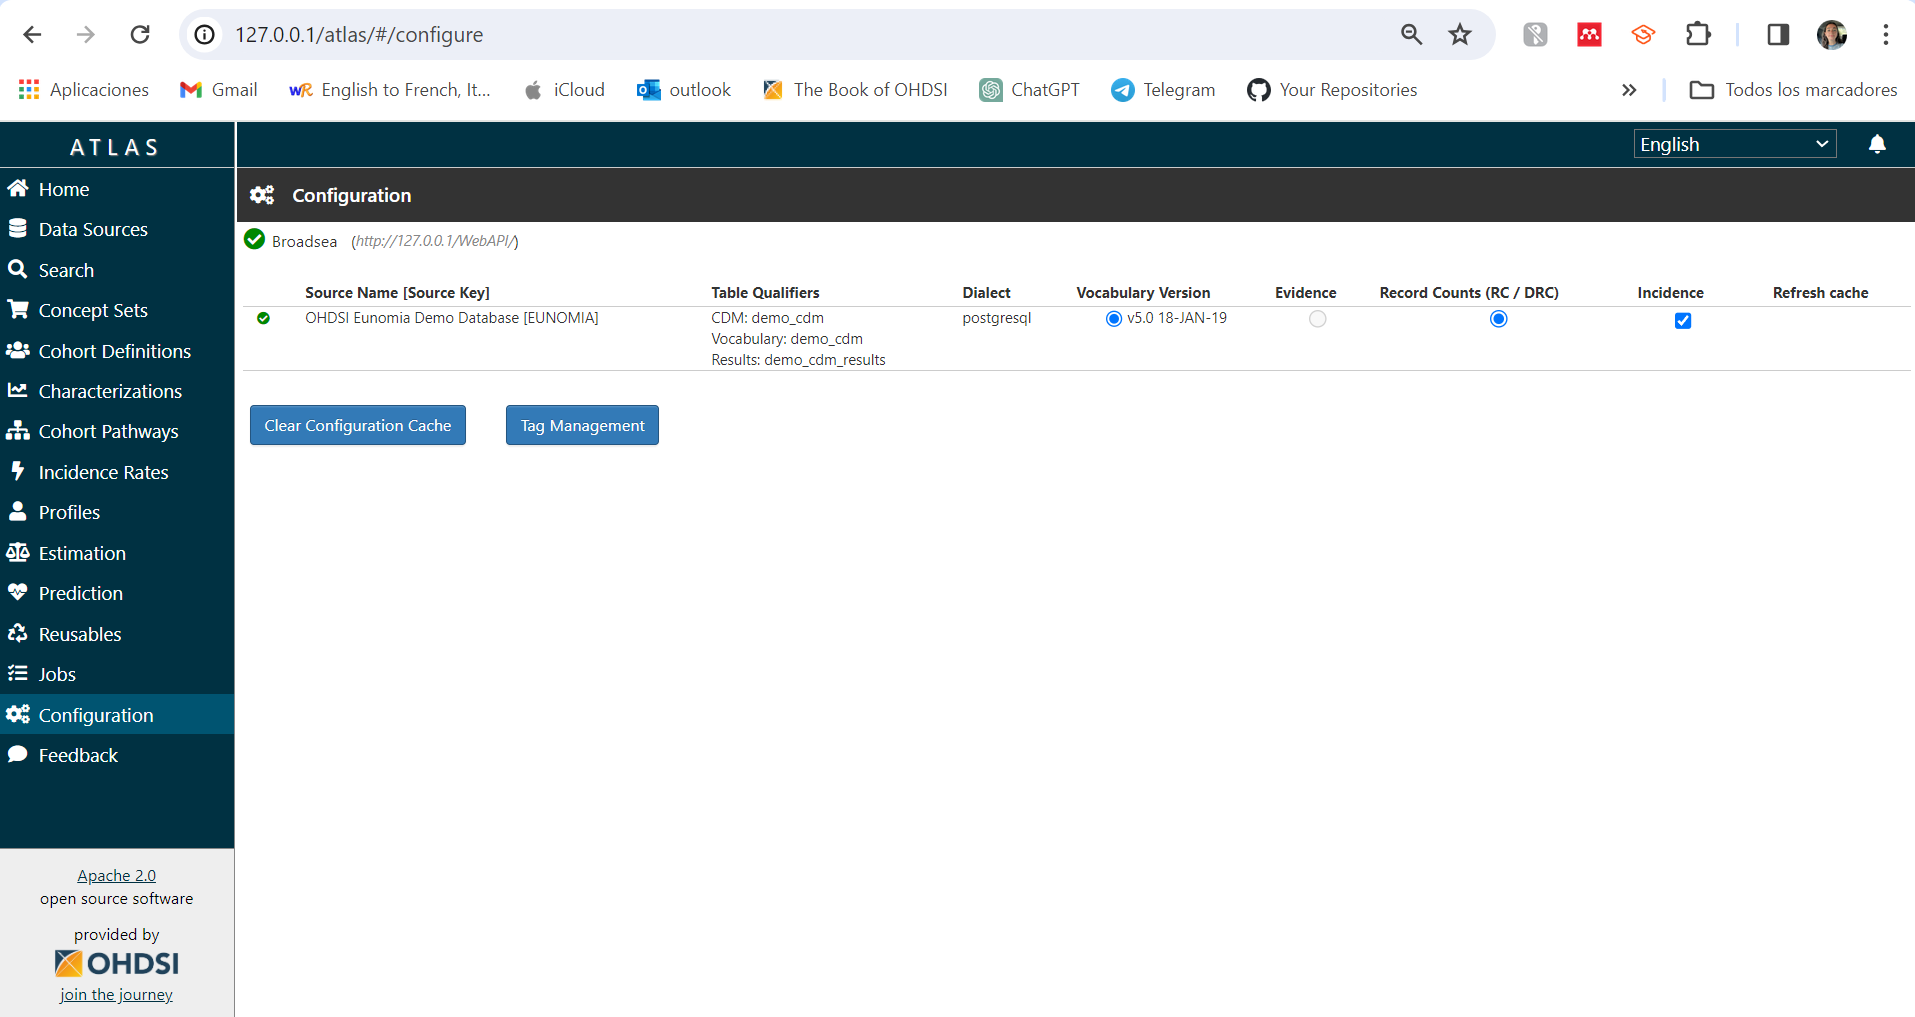
\includegraphics[width=0.90\textwidth]{figures/atlasBroadseaDB.png}
     \caption{Captura de pantalla de base de datos que utiliza ATLAS Broadsea}
    \label{fig:atlasBroadseaDB}
\end{figure}

    Por otra parte, y en contraste con la versión demo, ya no aparecen las entradas y estructuras que generan otros usuarios. La herramienta se presenta vacía, para ser completada solo con la información que nosotros introduzcamos.

\begin{figure}[H]
    \centering
    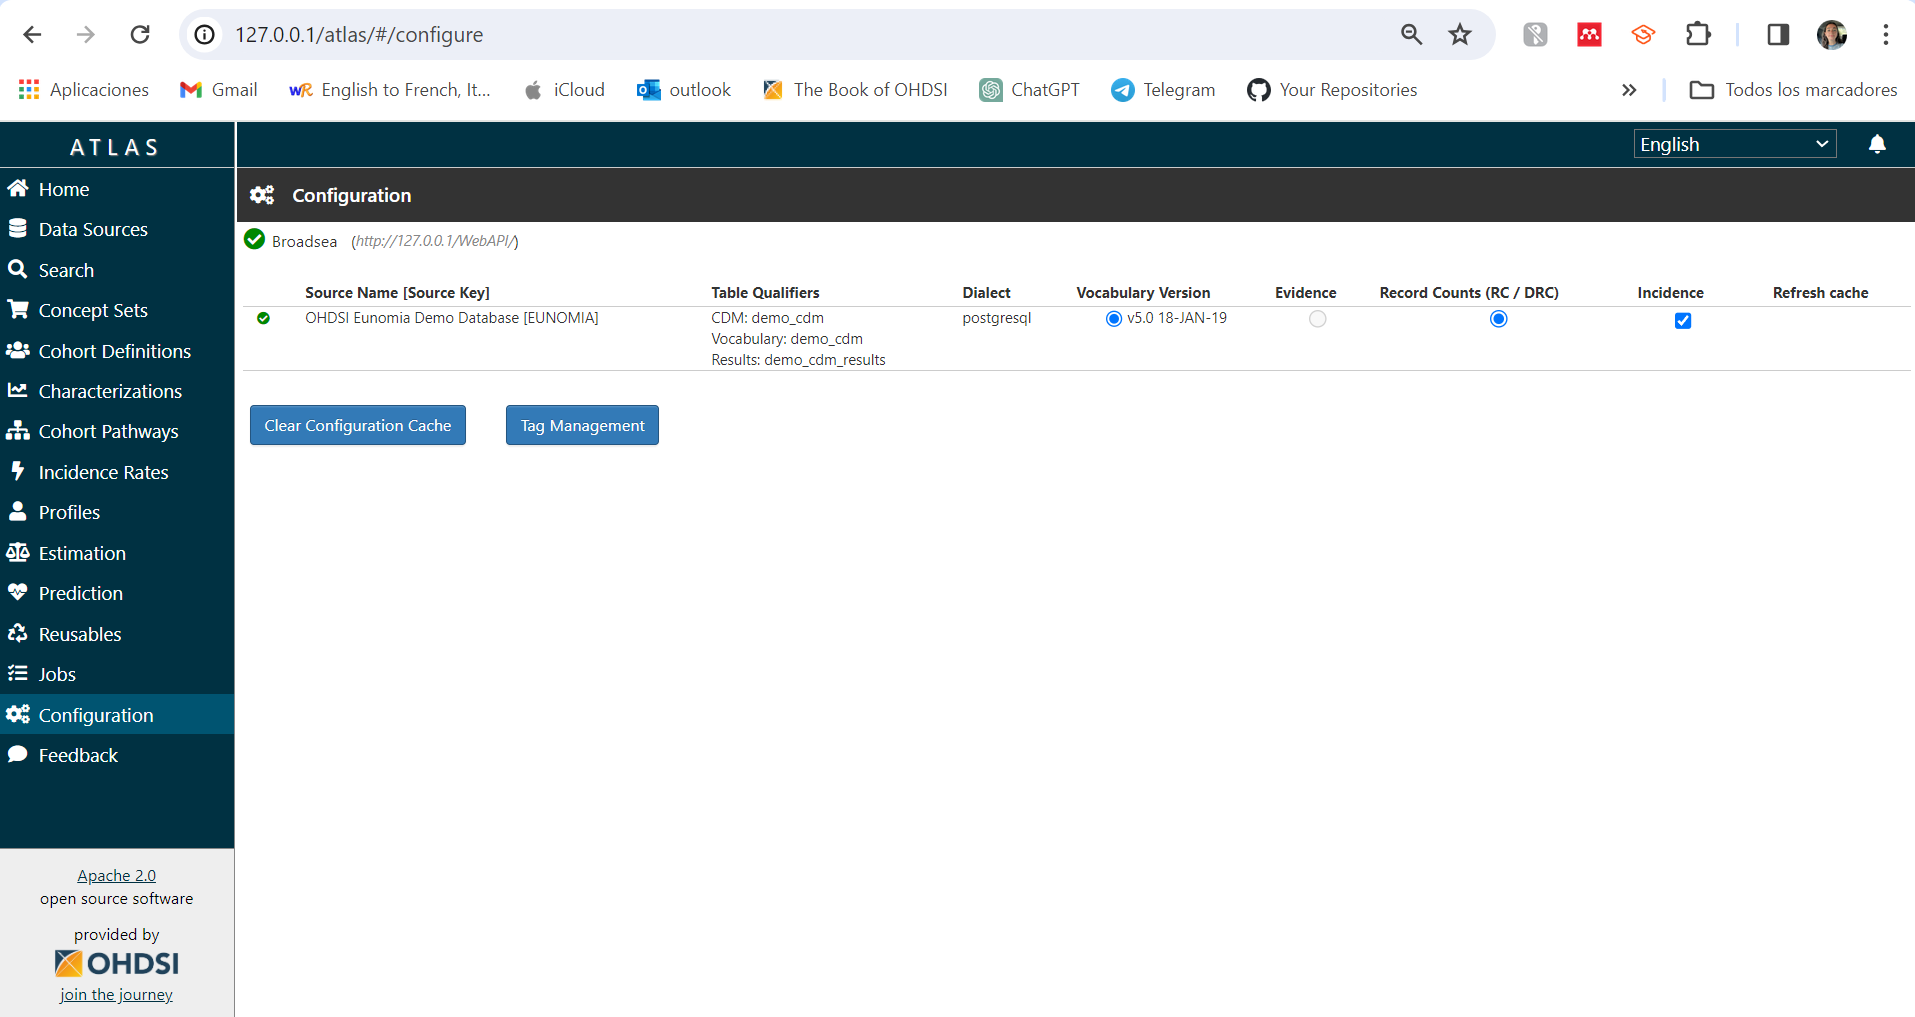
\includegraphics[width=0.90\textwidth]{figures/atlasBroadseaDB.png}
     \caption{Captura de pantalla señalando el número de entradas de definición de cohorte que almacena ATLAS Broadsea}
    \label{fig:atlasBroadseaDB}
\end{figure}
    
\end{enumerate}

\section{Solución de posibles errores}

\subsubsection{Error: Application initialization failed. Unable to connect to an instance of the WebAPI. Please contact your administrator to resolve this issue.}

El error aparece al dirigirse al servidor de Broadsea en el navegador.

\begin{figure}[H]
    \centering
    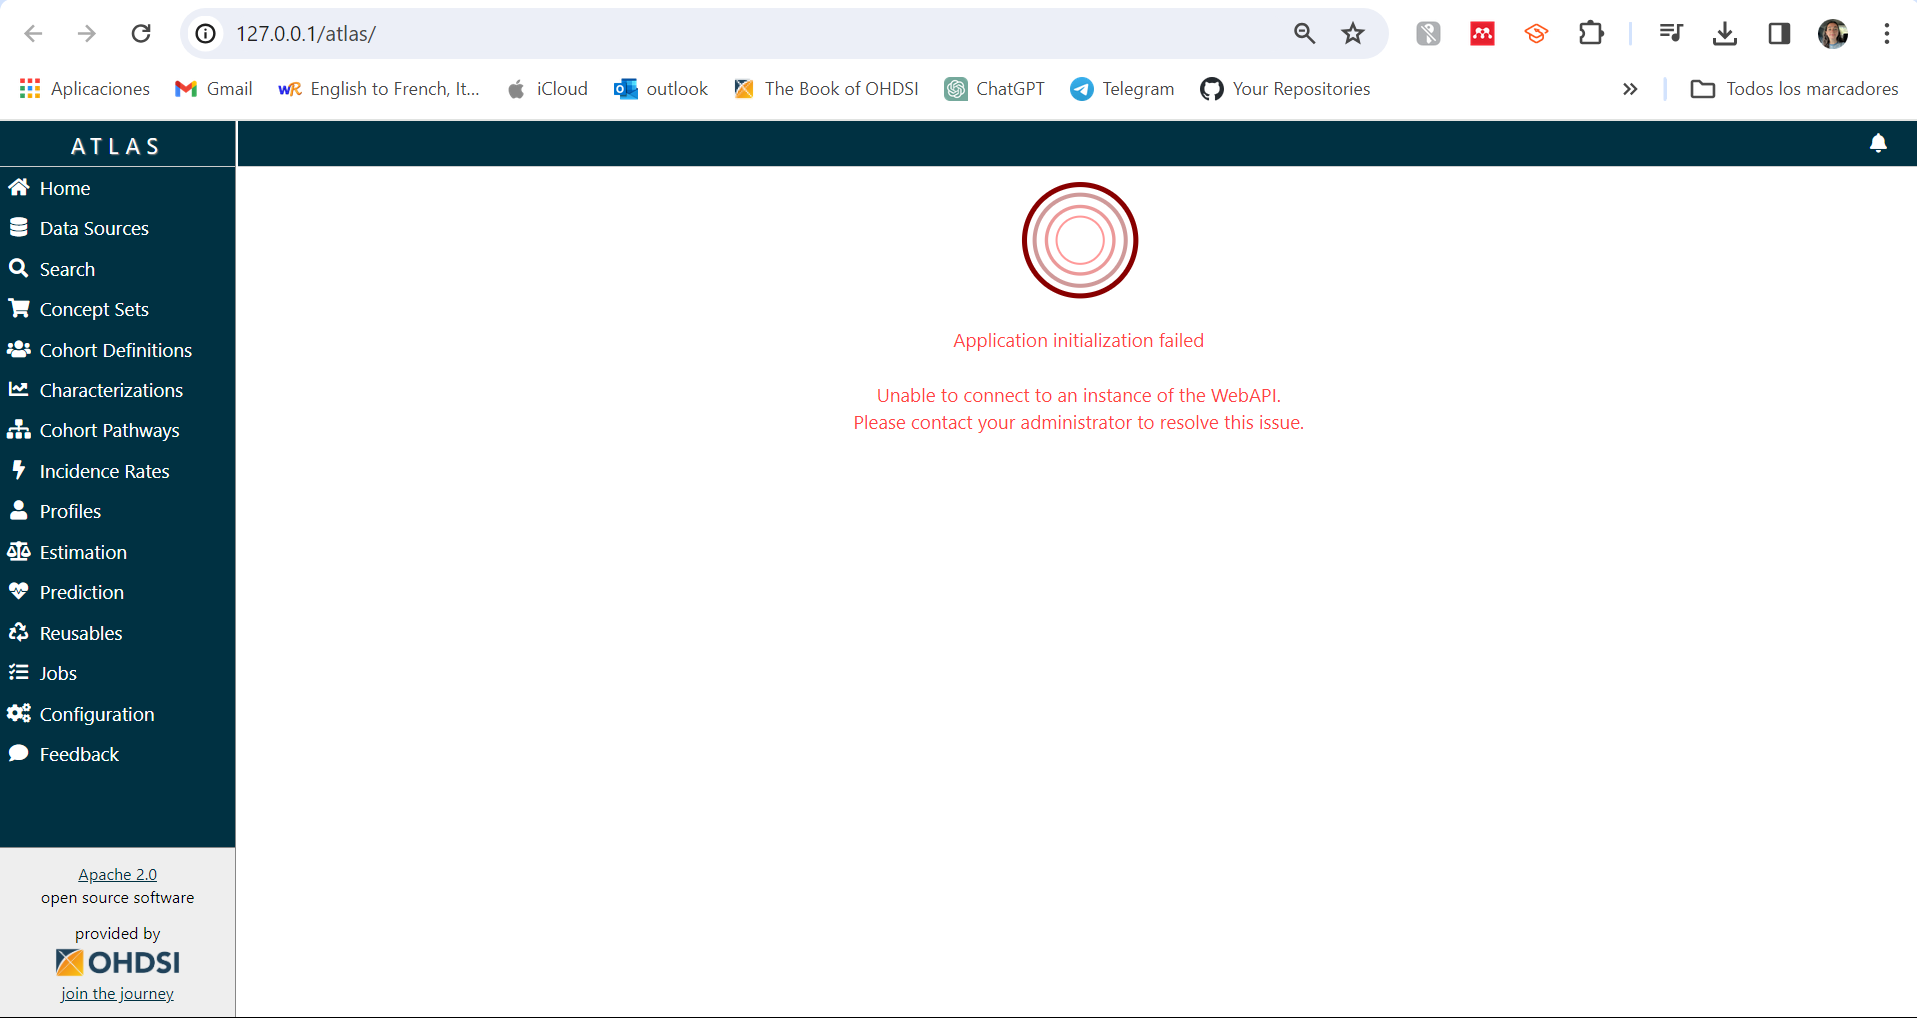
\includegraphics[width=0.90\textwidth]{figures/Error02AppFailed.png}
     \caption{Captura de pantalla del error}
    \label{fig:Error02AppFailed}
\end{figure}

Solución: Comprobar que todos los contenedores de docker implicados están corriendo


